As robotic applications flourish in our modern world, there is an increasing need for high reduction, high torque, and low backlash actuator systems.
These actuators are present in all types of robotic equipment and are critical in space flight applications.
A notable recent example includes the Curiosity rover from NASA's Jet Propulsion Laboratory that uses 33 separate motors with various reductions \cite{curiosity}.
Currently, harmonic drives are the primary reduction method when high ratio and compact design are required.
Commercially, these reducers come in limited reduction ratio options, and require a substantial amount of additional mass to withstand high torque applications.
Ideally, one would be able to specify a desired reduction ratio and realize it in a compact, lightweight package.

\begin{figure*}[t]
	\centering
	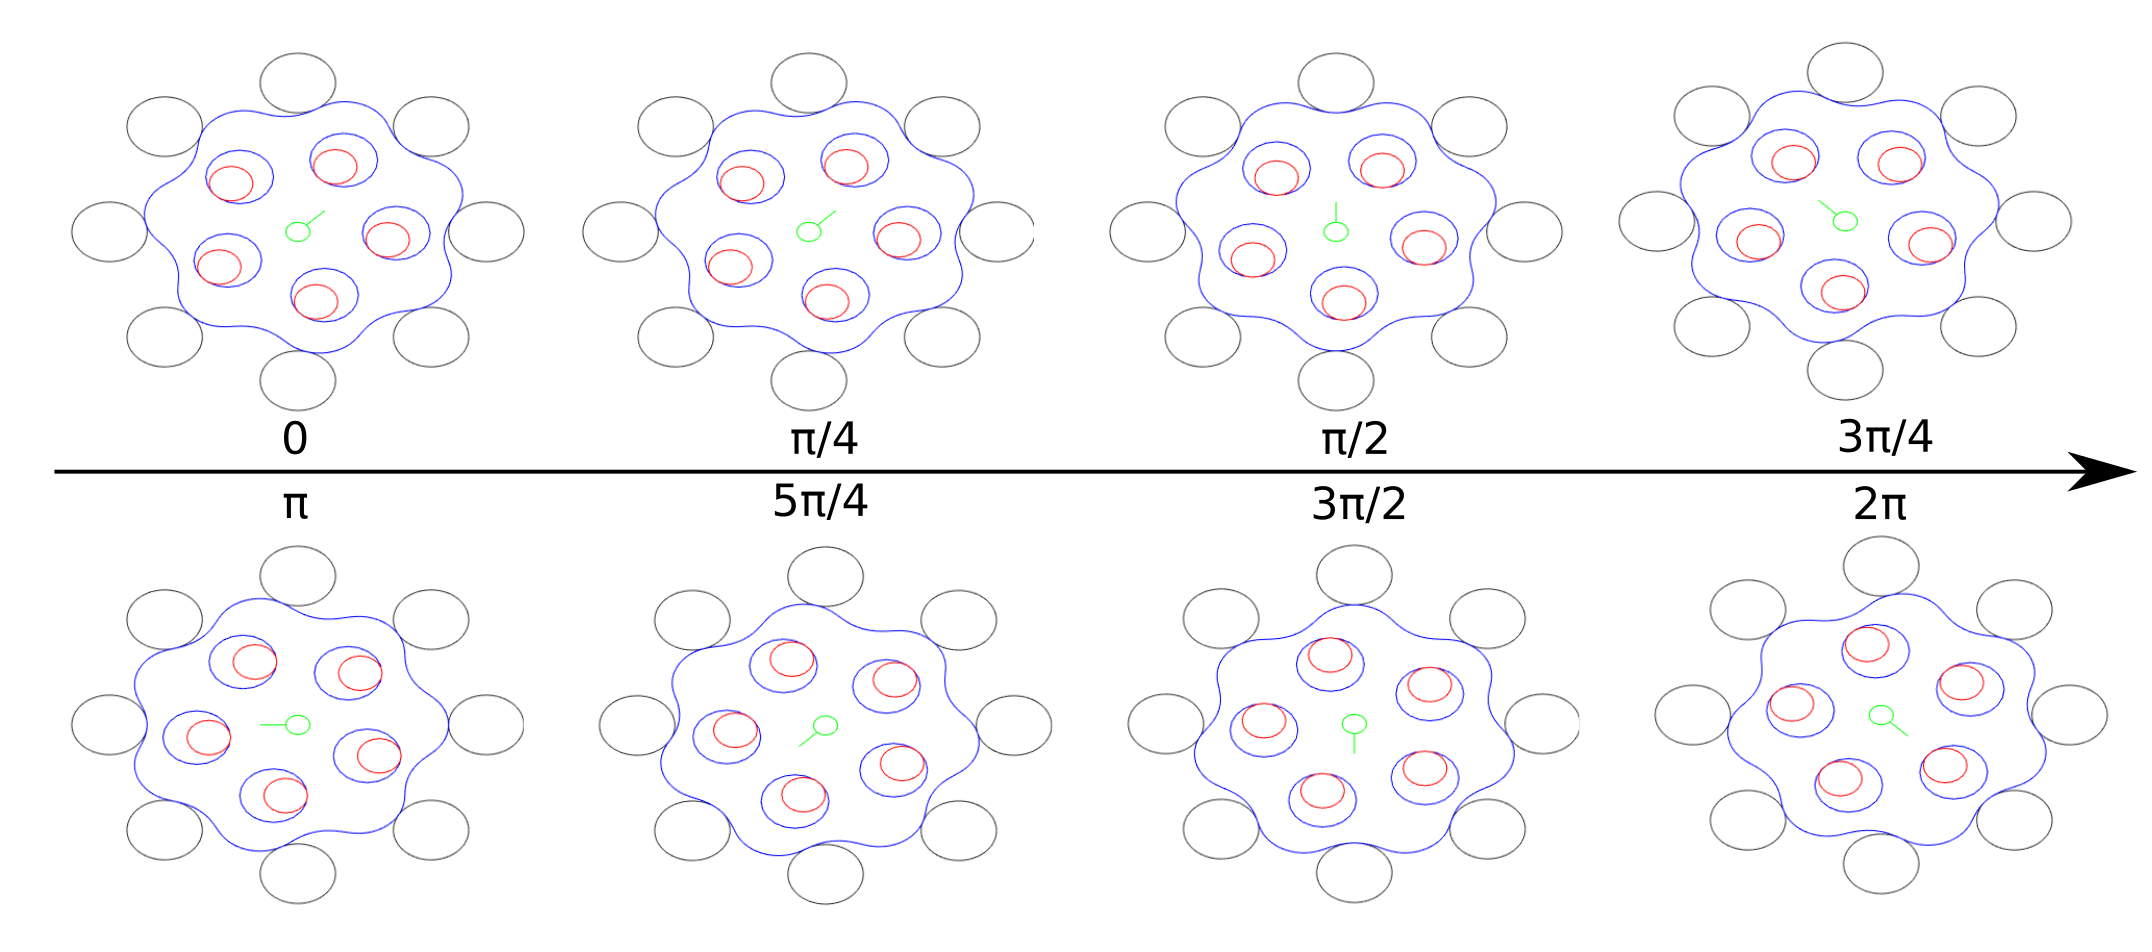
\includegraphics[width=0.8\linewidth]{images/single_motion}
	\caption{An example of a cycloid actuators motion with eight housing pins (black), seven lobes (blue) for a ratio of 7:1 and fie output pins (red). A single input revolution of the green input shaft is shown, resulting in 1/7 counter-rotation of the cycloid plate. This counter-rotation presses against the red pins, resulting in the output counter-rotation. 
	}
	\label{cycloid_motion}
\end{figure*}

\subsection{Cycloidal Drive Motivation}

Cycloidal drives are potentially an apt replacement for these harmonic drives as they can offer a large reduction in a small package, with large being defined as requiring three or more stages in a typical planetary drive. 
In situations where small backlash is acceptable, generally less than 30 arc-minutes, cycloids offer distinct advantages.

\begin{enumerate}
\item
They can be customized into the system directly. They allow specific reductions and load selection and can be incorporated directly into the actuator housing.
\item
They are made of relatively easy to manufacture parts compared to a harmonic drive.
\item
The torque to weight ratio typically higher for cycloidal drives of this style over a harmonic drive.
For example, the cycloid presented in this work is 2.5kg including all housing components, while a comparable harmonic drive is 5.1kg.
\end{enumerate}

Cycloidal drives have many desirable characteristics. These characteristics are covered well on a theoretical basis in the literature. However, these actuators are commonly used in robotic actuator design, potentially due to the lack of data that is available about their in-use operation.

The primary contribution of this research is to quantify the efficiency of a cycloidal drive system through an extended drive cycle test for burn-in to steady state performance and efficiency over the torque/speed profile.
To date, the actuator has been subjected to over 51k output revolutions through over 100 hours.

\begin{figure}[!b]
   \centering
   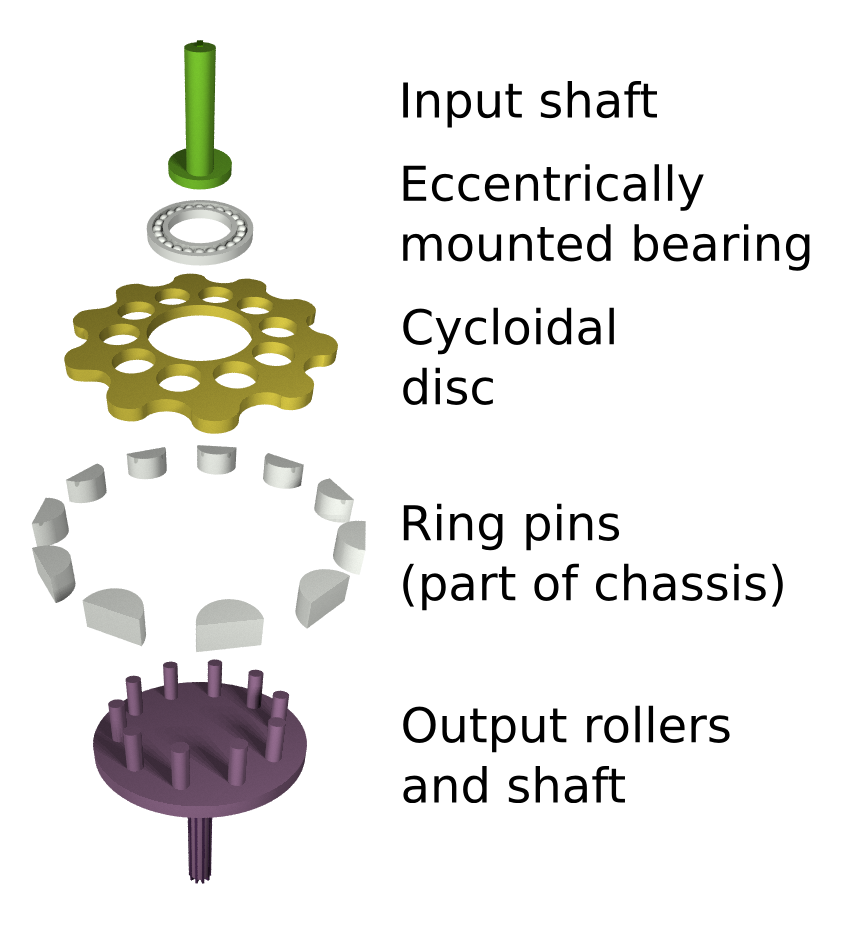
\includegraphics[width=0.60\linewidth]{images/Cycloidal_drive_parts}
    \caption{Simple rendering of the key elements that create a cycloidal drive.
   	A drive shaft spins a cycloidal disk via an eccentric circle (green).
   	The cycloid plate (yellow) reacts against the housing pins (gray) to create a counter-rotation, harnessed by the output pins (purple). (Public domain image from \cite{cycloid_cartoon})}
   \label{cycloid_cartoon}
\end{figure}



\subsection{Cycloidal Drive Background}
Cycloidal drives were proposed as early as 1956 by Botsiber and Kingston \cite{1956}.
The premise of this design leverages a plate, referred to as the cycloid plate, with lobes that interact with pins in the housing being spun on an eccentric shaft with a bearing.
The interaction between the eccentric rotation and the lobes pressing between the pins induces a counter-clockwise motion of the plate. This counter-clockwise rotation is harnessed via the interior pins that connect to a concentric plate that acts as the output of the mechanism (seen in Fig \ref{cycloid_cartoon}). A graphic of this motion, Fig \ref{cycloid_motion}, shows how the cycloid moves through a single input revolution causing 1/7 of an output revolution through the output pins. 
The reduction equation \ref{eq:single_stage_ratio} gives the overall reduction of the single-stage cycloid where \textit{N\textsubscript{lobes}} is the number of lobes on the cycloid plate and \textit{N\textsubscript{pins}} is the number of pins in the housing. 

\begin{equation} \label{eq:single_stage_ratio}
Q = \frac{N_{lobes}} {N_{pins} - N_{lobes}}
\end{equation}

This geartrain design has been used in industry for high torque, high shock load applications for many years including companies like Nabtesco Motion Control.
However, in many of these applications, many or all of the interacting surfaces like the housing pins and output pins use needle roller bearings to transmit load.
This allows for higher efficiency and load carrying capability, but it also increases mass and volume.
In the robotic industry, groups are striving to reduce the mass and volume of these actuators while still achieving high reduction and load capabilities.
One method for reducing mass is eliminating the rolling elements at the interaction points between the cycloid plate, housing pins, and output pins.
This allows for very compact and strong designs to be considered, but leaves the potential for larger losses and shorter system lifetime.

Many works have been presented on the subject of the theoretical design of these cycloidal drives \cite{on_the_lobe} \cite{hwang_hsieh}, designing with machine tolerances \cite{design_and_application}, contact and stress analysis \cite{li}, and performance characteristics such as torque ripple and backlash \cite{hsieh_traditional} \cite{hsieh_dynamics} as will be presented in Section \ref{design}.
These works lay a solid foundation for a designer, providing the equations and design considerations for a cycloid.
Still, there is a need to present in-use characteristics to support the theoretical calculations and models which has not been met in the current literature.

Theoretical cycloid efficiencies have been reported in the 88-98\% range \cite{Malhorta}, \cite{unified_approach}.
More recently, Sinsinger and Lipsey reported experimentally determined efficiencies for fused roller designs (42.3\%) and pin designs (71\%) based on 80 minutes of run-time \cite{cycloid_vs_harmonic}.
The distinction between a fused roller and pin design comes in the design of the housing.
In a fused design, the input pins are machined as part of the housing, and in a pin design, pins are inserted to ride in the housing, allowing relative motion.

Hsieh verified the stress present in the drives in simulation and in-use which demonstrated lower stress levels and torque ripple when using fused rollers \cite{hsieh_dynamics}.
These two results leave an open trade to designers if stress and torque ripple need to be minimized versus maximizing efficiency.

The aim of this work is to utilize a custom cycloid design for a NASA rover application and show the in-use efficiency characteristics over an extended duration test.
The actuator design is presented in Section \ref{design}.
A description of the experimental setup and procedure is provided in Section \ref{methods}.
Finally, the results and analysis of this high torque actuator and its implications are presented and discussed in Section \ref{results} and Section \ref{discussion}.

